\documentclass[12pt, a4paper]{article}
\usepackage[utf8]{inputenc}
\usepackage[T1]{fontenc}
\usepackage{pgfplots}
\usepackage{tikz}
\usetikzlibrary{angles}
\usetikzlibrary{quotes}
\usepackage{amssymb}
\usepackage{amsmath}
\usepackage{amsfonts}
\usepackage{graphicx}
\DeclareMathOperator{\tg}{tg}
\newcommand{\tgx}{\tg x}
\DeclareMathOperator{\ctg}{ctg}
\newcommand{\ctgx}{\ctg x}
\pgfplotsset{compat=1.18, width=10cm}

\begin{document}
\tableofcontents
\newpage
\section{Wprowadzenie do Rachunku Różniczkowego}
\subsection{Algebra}
\subsubsection{Wartość Bezwzględna}
Dla liczby x, wartość bezwzględna oznacza:
$$
|x| =
\begin{cases} 
  x & \text{jeśli } x \geq 0, \\
  -x & \text{jeśli } x < 0.
\end{cases}
$$
Dla $2$ liczb możemy wyznaczyć odległość pomiędzy nimi na osi liczbowej. Odległość jest zawsze liczbą dodatnią.
Aby obliczyć odległość pomiędzy a i b możemy skorzystać z następójących wzorów:
$$\left|a-b\right|$$
$$\left|b-a\right|$$
Aby obliczyć punkt równoległy od punktu $a$ i $b$ można wykorzystać następujący wzór:
$$p = \frac{a+b}{2}$$
\subsubsection{Równania z wartością bezwzględną}
Równanie z wartością bezwględną takie jak np. $\left|x-2\right|=5$ można rozwiązać na 3 sposoby:
\begin{itemize}
  \item Sposób algebraiczny jest jednym z najczęściej używanych sposobów do obliczania wartości bezwzględnej
      $$\left|x-2\right|=5$$
      $$x-2=5 \vee x-2=-5$$
      $$x=7\vee x=-3$$
\newpage
  \item Sposób geometryczny opiera się na graficznym przedstawieniu równania
    \begin{center}
      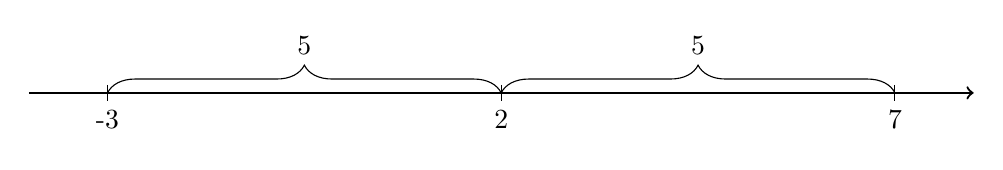
\begin{tikzpicture}
        \draw[thick, ->] (-4, 0) -- (8, 0);

        \foreach \x in {-3, 2, 7} {
          \draw (\x, 0.1) -- (\x, -0.1);
          \node[below] at (\x, -0.1) {\x};
        }
        \draw [decorate,decoration={brace,amplitude=10pt}] (-3,0) -- (2,0) node[midway,yshift=17pt] {5};
        \draw [decorate,decoration={brace,amplitude=10pt}] (2,0) -- (7,0) node[midway,yshift=17pt] {5};
        \node at (0, -0.5) {};
        \node at (0, 0.5) {};
      \end{tikzpicture}
    \end{center}
  \item Istnieje również sposób funkcyjny, który polega na narysowaniu funkcji po
        obu stronach równania i sprawdzeniu, dla jakich wartości zmiennych wyniki są
        równe. Ze względu na to, że ten sposób jest bardziej żmudny, a dwa wcześniejsze
        podejścia są bardziej efektywne, nie zostanie on przedstawiony graficznie w tym miejscu.
\end{itemize}
Warto również pamiętać aby nie liczyć równań których wynik równania z wartością bezwględną jest liczba ujemna np.
$$\left|x-2\right|\neq-5$$
\subsubsection{Nierówności z wartością bezwzględną}
\begin{itemize}
  \item Sposób algebraiczny.
      $$\left| x+2 \right| \leq 7$$
      $$x+2 \leq 7 \wedge x+2\geq -7$$
      $$x \leq 5 \wedge x \geq -9$$
      $$x \in \langle -9,5 \rangle$$

      $$\left| x-7 \right| > 2$$
      $$x-7 > 2 \vee x-7 < -2$$
      $$x > 9 \vee x < 5$$
      $$x \in \left(-\infty, 5\right) \cup \left(9, +\infty \right)$$
  %\item Sposób geometryczny opiera się na graficznym przedstawieniu równania
  %  \begin{center}
  %    \begin{tikzpicture}
  %      \draw[thick, ->] (-4, 0) -- (8, 0);
  %
  %      \foreach \x in {-3, 2, 7} {
  %        \draw (\x, 0.1) -- (\x, -0.1);
  %        \node[below] at (\x, -0.1) {\x};
  %      }
  %      \draw [decorate,decoration={brace,amplitude=10pt}] (-3,0) -- (2,0) node[midway,yshift=17pt] {5};
  %      \draw [decorate,decoration={brace,amplitude=10pt}] (2,0) -- (7,0) node[midway,yshift=17pt] {5};
  %      \node at (0, -0.5) {};
  %      \node at (0, 0.5) {};
  %   \end{tikzpicture}
  %  \end{center}
\end{itemize}
\subsection{Trygonometira}
W $\triangle$ prostokątnym dany jest kąt $\theta$. Wyraża się 4 funkcje trygonometryczne:
$$\sin\theta=\frac{a}{c}$$
$$\cos\theta=\frac{b}{c}$$
$$\tg\theta=\frac{a}{b}$$
$$\ctg\theta=\frac{b}{a}$$
\begin{center}
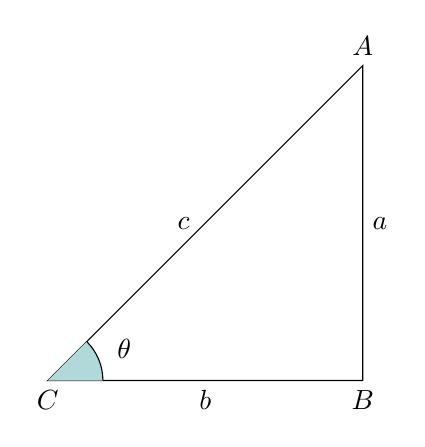
\begin{tikzpicture}
  \draw (0,0) coordinate[label=below:$C$] (c) --
        (4,0) coordinate[label=below:$B$] (b) node[midway, below] {$b$} --
        (4,4) coordinate[label=above:$A$] (a) node[midway, right] {$a$} --
        cycle node[midway, left=0.075cm] {$c$};
      \pic[draw, fill=teal!30, angle radius=7mm, "$\theta$", angle eccentricity=1.5] {angle = b--c--a};
\end{tikzpicture}
\end{center}
Funkcje trygonometryczne również posiadają tożsamości trygonometryczne takie jak np.
$$\sin^2\theta+\cos^2\theta = 1$$
$$\tg\theta=\frac{\sin\theta}{\cos\theta}$$
$$\ctg\theta=\frac{\cos\theta}{\sin\theta}$$
$$\tg\theta\cdot\ctg\theta=1$$
Funkcje trygonometryczne można konwertować na inne funkcje:
$$\sin(90^{\circ}-\theta)=\cos\theta$$
$$\cos(90^{\circ}-\theta)=\sin\theta$$
$$\tg(90^{\circ}-\theta)=\ctg\theta$$
$$\ctg(90^{\circ}-\theta)=\tg\theta$$
\section{Rachunek różniczkowo-całkowy}
\section{Algebra liniowa}
\subsection{Wektory}
Wektor to uporządkowana para liczb. Jeśli wektor ma początek to jest to, wektor
zaczepiony który jest oznaczany symbolem $\overrightarrow{AB}$. Jeżeli dane są punkty
$A = (x_1,y_1)$ oraz $B = (x_2,y_2)$,
to współrzędne wektora $\overrightarrow{AB}$ określa wzór: $$\overrightarrow{AB} = [x_2-x_1,y_2-y_1]$$
Jeśli natomiast wektor nie ma początku to jest to wektor swobodny który
jest oznaczany symbolem $\overrightarrow{v}, \overrightarrow{u}, \overrightarrow{w}$.
$$\overrightarrow{u} = \overrightarrow{w} \Longleftrightarrow u_x = w_x \wedge u_y = w_y$$
Na rysunku poniżej został przedstawiony wygląd wektora $[3,2]$ i $[-2,4]$ w układzie współrzędnych:

\begin{center}
\begin{tikzpicture}
\begin{axis}[xmin=-4.5,xmax=4.5,ymin=-2.5,ymax=4.5,axis lines=middle,
            xtick={-4,-3,...,4},ytick={-4,-3,...,4}, xlabel=$x$, ylabel=$y$,
            ]
  \addplot[domain=0:4, samples=250, ultra thick,blue, ->] coordinates {
    (0,0)
    (3,2)
  }
  node[pos=1.0, above left, blue]{$[3,2]$};
  \addplot[domain=0:4, samples=250,dashed] coordinates {
    (0,2)
    (3,2)
    (3,0)
  };

  \addplot[domain=0:4, samples=250, ultra thick,red, ->] coordinates {
    (0,0)
    (-2,4)
  }
  node[pos=1.0, below left, red]{$[-2,4]$};
  \addplot[domain=0:4, samples=250,dashed] coordinates {
    (0,4)
    (-2,4)
    (-2,0)
  };

\end{axis}
\end{tikzpicture}
\end{center}
Długość wektora $\overrightarrow{w}$ oraz $\overrightarrow{AB}$ można zapisać następująco:
$$|\overrightarrow{w}| = \sqrt{w^2_x + w^2_y}$$
$$|\overrightarrow{AB}| = \sqrt{\left(x_2 - x_1\right)^2 \left(y_2 - y_1\right)^2}$$
gdzie:
\begin{itemize}
  \item $A(x_1,y_1)$ i $B(x_2,y_2)$ to długości wektora $\overrightarrow{AB}$
\end{itemize}
\vspace{1em}
Sumą, różnicą, iloczynem $\overrightarrow{u} = [u_x,u_y]$ i $\overrightarrow{w} = [w_x,w_y]$, wyraża się wzorem:
$$\overrightarrow{u} + \overrightarrow{w} = [u_x + w_x, u_y + w_y]$$
\begin{center}
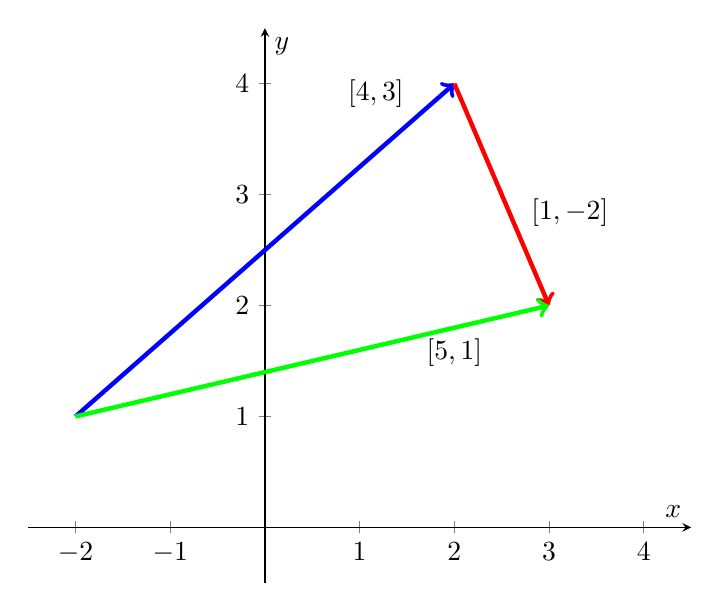
\begin{tikzpicture}
\begin{axis}[xmin=-2.5,xmax=4.5,ymin=-0.5,ymax=4.5,axis lines=middle,
            xtick={-4,-3,...,4},ytick={-4,-3,...,4}, xlabel=$x$, ylabel=$y$,
            ]
  \addplot[domain=0:4, samples=250, ultra thick,blue, ->] coordinates {
    (-2,1)
    (2,4)
  }
  node[pos=1.0, above = -0.125cm, left = 0.50cm, black]{$[4,3]$};
  \addplot[domain=0:4, samples=250, ultra thick,red, ->] coordinates {
    (2,4)
    (3,2)
  }
  node[pos=0.9, above = 0.9cm, right = -0.25cm, black]{$[1,-2]$};
  \addplot[domain=0:4, samples=250, ultra thick,green, ->] coordinates {
    (-2,1)
    (3,2)
  }
  node[pos=0.8, below, black]{$[5,1]$};
\end{axis}
\end{tikzpicture}
\end{center}
$$\overrightarrow{u} - \overrightarrow{w} = [u_x - w_x, u_y - w_y]$$

\begin{center}
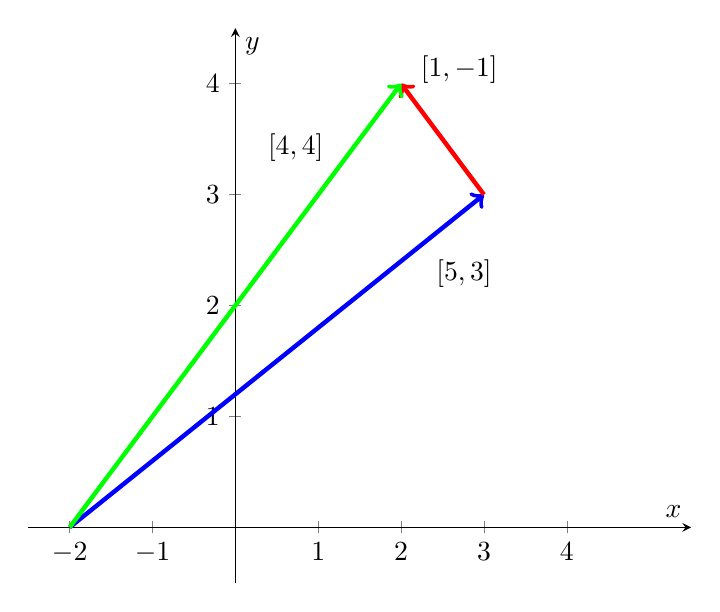
\begin{tikzpicture}
\begin{axis}[xmin=-2.5,xmax=5.5,ymin=-0.5,ymax=4.5,axis lines=middle,
            xtick={-4,-3,...,4},ytick={-4,-3,...,4}, xlabel=$x$, ylabel=$y$,
            ]
  \addplot[domain=0:4, samples=250, ultra thick,blue, ->] coordinates {
    (-2,0)
    (3,3)
  }
  node[pos=1.0, below = 1cm, right = -0.75cm, black]{$[5,3]$};

  \addplot[domain=0:4, samples=250, ultra thick,red, ->] coordinates {
    (3,3)
    (2,4)
  }
  node[pos=0.9, above right, black]{$[1,-1]$};

  \addplot[domain=0:4, samples=250, ultra thick,green, ->] coordinates {
    (-2,0)
    (2,4)
  }
  node[pos=0.8, above left, black]{$[4,4]$};
\end{axis}
\end{tikzpicture}
\end{center}
$$ a \cdot \overrightarrow{w} = [a \cdot w_x, a \cdot w_y], \quad \text{gdzie } a \in \mathbb{R}$$
\begin{center}
\begin{tikzpicture}
\begin{axis}[xmin=-3.5,xmax=2.5,ymin=-3.5,ymax=2.5,axis lines=middle,
            xtick={-4,-3,...,4},ytick={-4,-3,...,4}, xlabel=$x$, ylabel=$y$,
            ]
  \addplot[domain=0:4, samples=250, ultra thick,blue, ->] coordinates {
    (0,0)
    (1,1)
  }
  node[pos=1.0, above right, black]{$[5,3]$};

  \addplot[domain=0:4, samples=250, ultra thick,red, ->] coordinates {
    (0,0)
    (-2,-2)
  }
  node[pos=0.9, below left = 0.25cm, black]{$[-2,-1]$};
\end{axis}
\end{tikzpicture}
\end{center}
Wektory $\overrightarrow{u} = [u_x, u_y]$ i $\overrightarrow{w} = [w_x, w_y]$, są przeciwne wtedy,
gdy suma wektorów $\overrightarrow{u}$ i $\overrightarrow{w}$ jest wektorem zerowym, czyli:
$$\overrightarrow{u} = -\overrightarrow{w} \Longleftrightarrow u_x + w_x = 0 \wedge u_y + w_y = 0$$
\newline
Iloczyn skalarny wektorów $\overrightarrow{u} = [u_1,u_2]$ i $\overrightarrow{w} = [w_1,w_2]$ to liczba, którą można uzyskać
dodając iloczyny odpowiednich współrzędnych:
$$\overrightarrow{u} \cdot \overrightarrow{w} = u_1 \cdot w_1 + u_2 \cdot w_2$$
Iloczyn skalarny wektorów można również wyliczyć znając długości wektorów $|\overrightarrow{u}|$ i $|\overrightarrow{w}|$
oraz kąt $\theta$ między nimi:
$$\overrightarrow{u} \cdot \overrightarrow{w} = |\overrightarrow{u}| \cdot |\overrightarrow{w}| \cdot \cos \theta$$
\begin{center}
\begin{tikzpicture}
\begin{axis}[xmin=-3.5,xmax=3.5,ymin=-0.5,ymax=3.5,axis lines=middle,
            xtick={-4,-3,...,4},ytick={-4,-3,...,4}, xlabel=$x$, ylabel=$y$,
            ]
  \addplot[domain=0:4, samples=250, ultra thick,blue, ->] coordinates {
    (-2,1)
    (1,3)
  }
  node[pos=1.0, below right, black]{$[3,2]$};

  \addplot[domain=0:4, samples=250, ultra thick,red, ->] coordinates {
    (-2,1)
    (3,1)
  }
  node[pos=0.9, above left, black]{$[5,0]$};
\end{axis}
\end{tikzpicture}
\end{center}
\subsection{Przesunięcie równoległe wzdłuż osi OX i OY}
Przesunięcie wykresu funkcji najłatwiej jest zapisywać w postaci wektora przesunięcia:
$$\overrightarrow{u} = [1,5]$$
$$\overrightarrow{w} = [-2,-4]$$
Wektor $\overrightarrow{u} = [1,5]$ oznacza przesunięcie wykresu funkcji o 1 jednostke w prawą stronę
i 5 jednostki do góry, natomiast wektor $\overrightarrow{w} = [-2,-4]$
oznacza przesunięcie o jednostek 2 do lewej i 4 jednostki w dół. Na wykresie poniżej zostało przedstawione przesunięcie funkcji o
wektor $\overrightarrow{u} = [1,5]$.
\begin{center}
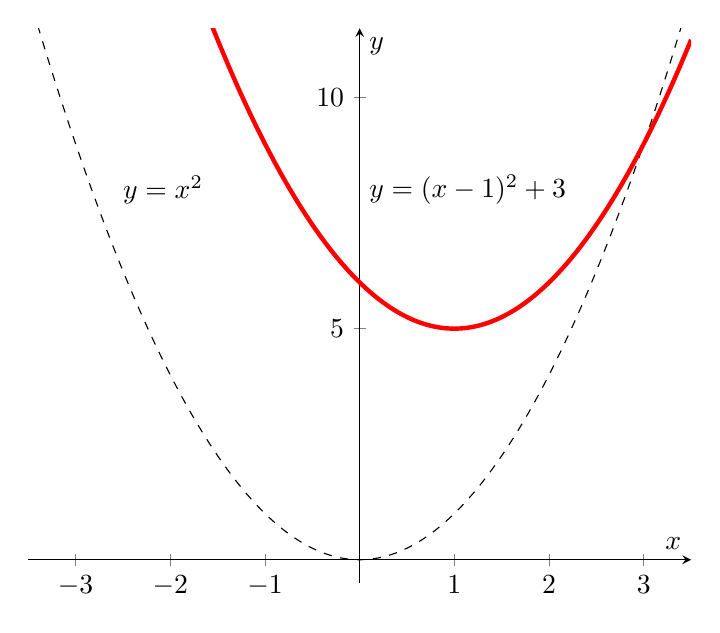
\begin{tikzpicture}
\begin{axis}[xmin=-3.5,xmax=3.5,ymin=-0.5,ymax=11.5,axis lines=middle,
            xtick={-4,-3,...,4},ytick={0,5,10}, xlabel=$x$, ylabel=$y$,
            ]
    \addplot[domain=-3.5:3.5, samples=250, dashed, black] {x^2};
    \node[anchor=west, black] at (axis cs:-2.6,8) {$y = x^2$};
    \addplot[domain=-3.5:3.5, samples=250, ultra thick, red] {(x-1)^2 + 5};
    \node[anchor=west, black] at (axis cs:0,8) {$y = (x-1)^2 + 3$};
\end{axis}
\end{tikzpicture}
\end{center}
Ogólny wzór przesunięcia funkcji o wektor $\overrightarrow{v} = [p, q]$ to:
$$g(x) = f\left(x - p\right) + q$$
\newpage
\subsection{Przekształcenie symetralne względem osi OX i OY}
Jeżeli wykres funkcji $y=f(x)$ odbijem symetrycznie względem osi $OX$, otrzymamy wykres funkcji $$y=-f(x)$$
\begin{center}
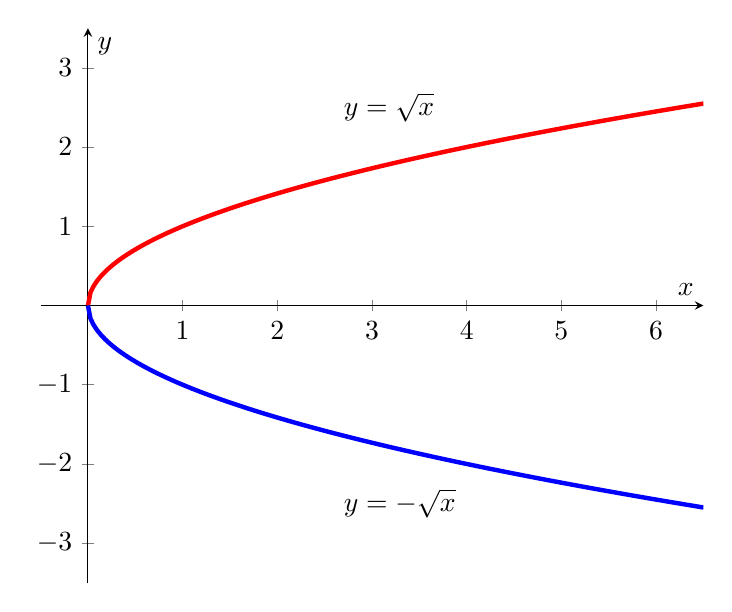
\begin{tikzpicture}
\begin{axis}[xmin=-0.5,xmax=6.5,ymin=-3.5,ymax=3.5,axis lines=middle,
            xtick={-10,...,10},ytick={-6,...,10}, xlabel=$x$, ylabel=$y$,
            ]
    \addplot[domain=0:6.5, samples=250, ultra thick, red] {sqrt(x)};
    \node[anchor=west, black] at (axis cs:2.6,2.5) {$y = \sqrt{x}$};
    \addplot[domain=0:6.5, samples=250, ultra thick, blue] {-sqrt(x)};
    \node[anchor=west, black] at (axis cs:2.6,-2.5) {$y = -\sqrt{x}$};
\end{axis}
\end{tikzpicture}
\end{center}
Jeżeli wykres funkcji $y=f(x)$ odbijem symetrycznie względem osi $OY$, otrzymamy wykres funkcji $$y=f(-x)$$
\begin{center}
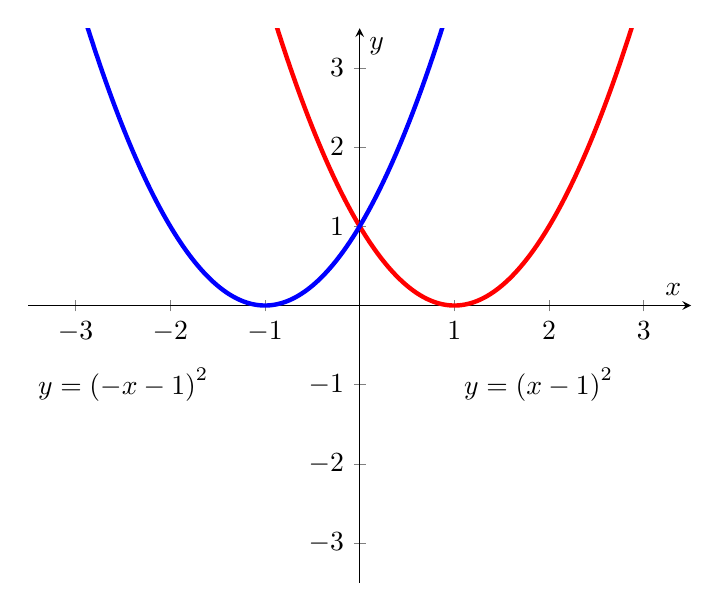
\begin{tikzpicture}
\begin{axis}[xmin=-3.5,xmax=3.5,ymin=-3.5,ymax=3.5,axis lines=middle,
            xtick={-10,...,10},ytick={-6,...,10}, xlabel=$x$, ylabel=$y$,
            ]
    \addplot[domain=-3:3, samples=250, ultra thick, red] {(x-1)^2};
    \node[anchor=west, black] at (axis cs:1,-1) {$y = \left(x-1\right)^2$};
    \addplot[domain=-3:3, samples=250, ultra thick, blue] {(-x-1)^2};
    \node[anchor=west, black] at (axis cs:-3.5,-1) {$y = \left(-x-1\right)^2$};
\end{axis}
\end{tikzpicture}
\end{center}
\end{document}
